\chapter{Bmad Concepts and Organization}
\label{c:lat.concepts}

This chapter is an overview of some of the nomenclature used
by \bmad. Presented are the basic concepts, such as \vn{element},
\vn{branch}, and \vn{lattice}, that \bmad uses to describe such things
as LINACs, storage rings, X-ray beam lines, etc.  

%---------------------------------------------------------------------------
\section{Lattice Elements}
\label{s:element.def}

\index{lattice element}
\index{element}
\index{controller element}
The basic building block \bmad uses to describe a machine is the
\vn{lattice} \vn{element}. An element can be a physical thing that
particles travel ``through'' like a bending magnet, a quadrupole or a
Bragg crystal, or something like a \vn{marker} element (\sref{s:mark})
that is used to mark a particular point in the machine.  Besides
physical elements, there are \vn{controller} elements
(Table~\ref{t:control.classes}) that can be used for parameter control
of other elements.

Chapter~\sref{c:elements} lists the complete set of different element
types that \bmad knows about.

%---------------------------------------------------------------------------
\section{Lattice Branches}
\label{s:branch.def}

\index{branch}
The next level up from a \vn{lattice} \vn{element} is the \vn{lattice}
\vn{branch} (\sref{s:branch}). A \vn{lattice} \vn{branch} is not to
be confused with a \vn{branch} element (\sref{s:branch}). A
\vn{lattice} \vn{branch} is just an ordered sequence of lattice
elements that a particle will travel through. A branch can represent a
LINAC, X-Ray beam line, storage ring or anything else that can be
represented as a simple ordered list of elements.

Chapter~\sref{c:sequence} shows how a \vn{branch} is defined in a
lattice file with \vn{line}, \vn{list}, and \vn{use} statements.

\index{beginning element}\index{end element}
All elements in a branch are assigned a number starting from zero. The
zeroth \vn{init_ele} (\sref{s:init.ele}) element, which is always
named \vn{BEGINNING}, is automatically included in every branch and is
used as a marker for the beginning of the branch.  Additionally, every
branch will, by default, have a final marker element (\sref{s:mark})
named \vn{END}.

%---------------------------------------------------------------------------
\section{Lattice}
\label{s:lattice.def}

\index{lattice}\index{branch} 
A \vn{lattice} is just an array of \vn{branches} that can be
interconnected together to describe an entire machine complex.  The
array of \vn{branches} in a \vn{lattice} is numbered starting from
zero. A \vn{lattice} can include such things as transfer lines, dump
lines, x-ray beam lines, colliding beam storage rings, etc. All of
which are connected together to form a coherent whole. In addition, a
lattice may contain \vn{controller elements} (Table~\ref{t:control.classes}) which
can simulate such things as magnet power supplies and lattice element
mechanical support structures.

\index{root branch}
Branches can be interconnected using \vn{branch} and
\vn{photon_branch} elements (\sref{s:branch}). This is used to
simulate forking beam lines (\sref{s:branch}) such as a connections
to a transfer line, dump line, or an X-ray beam line. The \vn{branch}
from which other \vn{branches} fork is called a \vn{root} branch.

A lattice may contain multiple \vn{root} \vn{branches}. For example, a
pair of intersecting storage rings will generally have two \vn{root}
branches, one for each ring. The \vn{use} statement (\sref{s:use}) in a
lattice file will list the \vn{root} \vn{branches} of a lattice. To
connect together lattice elements that are physically shared between
branches, for example, the interaction region in colliding beam
machines, \vn{multipass} lines (\sref{s:multipass}) can be used.

%---------------------------------------------------------------------------
\section{Lord and Slave Elements}
\label{s:lord.slave}

\begin{figure}[tb]
 \begin{center}
 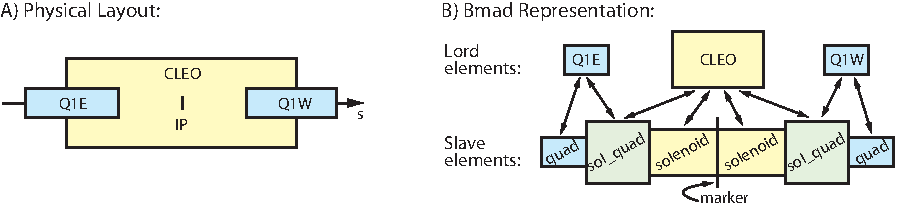
\includegraphics[width=6.0in]{superimpose-ip.pdf}
 \caption[Superposition example.]
 {
Superposition Example. A) Interaction region layout
with quadrupoles overlapping a solenoid. B) The Bmad lattice
representation has a list of split elements to track through and the
undivided ``lord'' elements. Pointers (double headed arrows), keep
track of the correspondence between the lords and their slaves.
 }
 \label{f:super.ip}
 \end{center}
 \end{figure}

%---------------------------------------------------------------------------

A real machine is more than a collection of independent lattice
elements. For example, the field strength in a string of elements may
be tied together via a common power supply, or the fields of different
elements may overlap.

\bmad tries to capture these interdependencies using what are referred
to as \vn{lord} and \vn{slave} elements. The \vn{lord} elements may be
divided into two classes. In one class are the \vn{controller}
elements.  These are \vn{overlay} (\sref{s:overlay}), \vn{group}
(\sref{s:group}), and \vn{girder} (\sref{s:girder}) elements that
control the attributes of other elements which are their slaves.

The other class of \vn{lord} elements embody the separation of the
physical element from the track that a particle takes when it passes
through the element. There are two types


An example will make this clear.
\vn{Superposition} (\sref{s:super}) is the ability to overlap lattice
elements spatially. \fig{f:super.ip} shows an example which is a
greatly simplified version of the IR region of Cornell's CESR storage
ring when CESR was an e+/e-- collider. As shown in \fig{f:super.ip}A,
two quadrupoles named \vn{q1w} and \vn{q1e} are partially inside and
partially outside the interaction region solenoid named \vn{cleo}. In
the lattice file, the IR region layout is defined to be
 {\small
\begin{example}
  cesr: line = (... q1e, dft1, ip, dft1, q1w ...)
  cleo: solenoid, l = 3.51, superimpose, ref = ip
\end{example}
 }
The line named \vn{cesr} ignores the solenoid and just contains the
interaction point marker element named \vn{ip} which is surrounded by
two drifts named \vn{dft1} which are, in turn, surrounded by the
\vn{q1w} and \vn{q1e} quadrupoles. The solenoid is added to the layout
on the second line by using superposition. The ``ref = ip'' indicates
that the solenoid is placed relative to \vn{ip}. The default, which is
used here, is to place the center of the superimposed \vn{cleo}
element at the center of the \vn{ip} reference element.  The
representation of the lattice in \bmad will contain two branch
\vn{sections} (``sections'' is explained more fully later): One
section, called the \vn{tracking section}, contains the elements that
are needed for tracking particles. In the current example, as shown in
\fig{f:super.ip}B, the first IR element in the tracking section is a
quadrupole that represents the part of \vn{q1e} outside of the
solenoid. The next element is a combination solenoid/quadrupole,
called a \vn{sol_quad}, that represents the part of \vn{q1e} inside
\vn{cleo}, etc.  The other branch section that Bmad creates is called
the \vn{lord section} This section contain the undivided ``physical''
\vn{super_lord} elements (\sref{s:super}) which, in this case are
\vn{q1e}, \vn{q1w}, and \vn{cleo}. Pointers are created between the
lords and their \vn{super_slave} elements in the tracking section so
that changes in parameters of the lord elements can be transferred to
their corresponding slaves.

\vn{super_lord}s are used when there are overlapping fields between
elements, the other case where there is a separation between the
physical element and the particle track comes when a particle passes
through the same physical element multiple times such as in an Energy
Recovery Linac or where different beams pass through the same element
such as in an interaction region. In this case, \vn{multipass_lords}
representing the physical element and \vn{multipass_slaves}
representing the track can be constructed (\sref{s:multipass}).
Superposition and multipass can be combined in situations where there
are overlapping fields in elements where the particle passes through

For historical reasons, each \vn{branch} in a lattice has a
\vn{tracking section} and a \vn{lord section} and the \vn{tracking
section} is always the first (lower) part of the element array and the
\vn{lord section} inhabits the second (upper) part of the array.  All
the \vn{lord} elements are put in the \vn{lord section} of branch 0
and all the other \vn{lord sections} of all the other branches are
empty.

As a side note, Etienne Forest's PTC code (\sref{s:ptc.intro}) uses separate
structures to separate the physical element, which PTC calls an
\vn{element} from the particle track which PTC call a \vn{fibre}.
[Actually, PTC has two structures for the physical element,
\vn{element} and \vn{elementp}. The latter being the ``polymorph''
version.] This \vn{element} and \vn{fibre} combination corresponds to
\bmad \vn{multipass_lord} and \vn{multipass_slave} elements. PTC does
not handle overlapping fields as \bmad does with \vn{superposition}
(\sref{s:super}).

%---------------------------------------------------------------------------
\section{PTC: Polynomial Tracking Code}
\label{s:ptc.intro}
\index{PTC}

Etienne Forest\cite{b:forest} has written what is actually two
software libraries: FPP and PTC.  FPP stands for ``Fully Polymorphic
Package.'' What this library does is implement Taylor maps (aka
Truncated Power Series Algebra or TPSA) and Lie algebraic
operations. Thus in FPP you can define a Hamiltonian and then generate
the Taylor map for this Hamiltonian. FPP is very general. It can work
with an arbitrary number of dimensions.  FPP, however, is a purely
mathematical package in the sense that it knows nothing about
accelerator physics. That is, it does not know about bends,
quadrupoles or any other kind of element, it has no conception of a
lattice (a string of elements), it doesn't know anything about Twiss
parameters, etc. This is where PTC (Polymorphic Tracking Code) comes
in. PTC implements the high energy physics stuff and uses FPP as
the engine to do the Lie algebraic calculations.  For the purposes of
this manual, PTC and FPP are generally considered one package and the
combined PTC/FPP will be referred to as simply ``PTC''.
For programmers, interface documentation can be found in
chapter~\sref{c:ptc}.

\index{PTC!single element mode}
\bmad interfaces to PTC in two ways: One way, called ``single
element'' mode, uses PTC on a per element basis. In this case, the
method used for tracking a given element can be selected on an
element-by-element basis so non-PTC tracking methods can be mixed with
PTC tracking methods to optimize speed and accuracy. [PTC tends to be
accurate but slow.] The advantage of single element mode is the
flexibility it affords. The disadvantage is that it precludes using
PTC's analysis tools which rely on the entire lattice being tracked
via PTC. Such tools include normal form analysis beam envelope
tracking, etc.

\index{PTC!whole lattice mode}
The alternative to single element mode is ``whole lattice'' mode where
a series of PTC \vn{layout}s (equivalent to a \bmad branch) are
created from a \bmad lattice. Whether single element or whole lattice
mode (or both) is used is determined by the program being run.

